\documentclass[11pt,a4paper]{article}


\setlength{\topmargin}{-55pt}%
\setlength{\oddsidemargin}{-20pt}%
\setlength{\textwidth}{490pt}%
\setlength{\textheight}{700pt}%
\setlength{\headsep}{20pt}%
\setlength{\headheight}{14pt}

\usepackage[utf8]{inputenc} % accents 8 bits dans le fichier
\usepackage[T1]{fontenc}      % accents codés dans la fonte
\usepackage[french]{babel}
\usepackage{amsmath,amssymb}
\usepackage{graphicx}
\usepackage{fancyhdr}
\usepackage{booktabs}
\usepackage{color, colortbl}
\usepackage{appendix}
\usepackage{pgfplots}
\usepackage[hidelinks]{hyperref}
\usepackage{siunitx}
\usepackage{algorithmicx}
\usepackage{algorithm}
\usepackage{algpseudocode}
\usepackage{subcaption}

\pgfplotsset{compat=1.3}

\addto\captionsfrench{% Replace "english" with the language you use
  \renewcommand{\contentsname}%
    {Table des matières}
}

\DecimalMathComma

\lhead{}      %en-tête
\chead{MPNA : Méthode des itérations simultanées}%
\rhead{}%
\lfoot{\tiny{Pierre GRANGER \& Matthias BEAUPERE}}
\cfoot{}%
\rfoot{\thepage}%
\renewcommand{\headrulewidth}{0.5pt}
\renewcommand{\footrulewidth}{0.5pt}
\pagestyle{fancy}

\newcommand{\HRule}{\rule{\linewidth}{0.5mm}}
\newcommand{\norm}[1]{\left\lVert#1\right\rVert}

\definecolor{green}{rgb}{0.2,0.8,0.2}

\begin{document}
\begin{center}

	{\LARGE\centering Projet de MPNA :\\ Méthode des itérations simultanées}\\[1cm]

	{ Matthias \bsc{Beaupère}, Pierre \bsc{Granger}}\\[0.5cm]
	{Rapport MPNA - CHPS - \today}\\[2cm]
\end{center}

\tableofcontents
\newpage

\section{Introduction et position du problème}
	De nombreux problèmes modernes impliquent le calcul de valeurs propres et de vecteurs propres de grandes matrices creuses. Souvent, on ne désire que les quelques valeurs propres dominantes de la matrice et on souhaite utiliser une méthode robuste et efficace. Par exemple, ce problème peut être rencontré lors de l'étude de certains systèmes physiques ou bien par exemple dans les moteurs de recherche qui reposent sur ce type de technique. Des algorithmes spécifiques doivent être utilisés afin de résoudre ces problèmes de valeur propre en un temps raisonnable. De plus les algorithmes utilisés doivent pouvoir être facilement utilisés sur les architectures massivement parallèles actuelles ce qui représente un grand défi.

\section{Approche utilisée}
	Afin d'effectuer le calcul d'un petit nombre de vecteurs propres dominants d'une grande matrice, on se propose d'implémenter en langage \textbf{C} l'algorithme des itérations simultanées aussi appelé algorithme d'itération du sous-espace.
	L'algorithme des itérations simultanées est basé sur la méthode de la puissance qui consiste à extraire la valeur propre principale d'une matrice en multipliant un grand nombre $N$ de fois un vecteur initial par la matrice d'intérêt $A$. On s'attend alors à voir converger le vecteur vers le vecteur propre dominant de $A$ à la vitesse $\left(\frac{\lambda_2}{\lambda_1}\right)^N$ avec $\lambda_1$ la valeur propre dominante et $\lambda_2$ la seconde valeur propre dominante.
	La méthode des itérations simultanées permet de calculer un espace invariant par $A$ de dimension $k > 1$ et ainsi d'extraire les $k$ valeurs propres dominantes plutôt qu'un seule. Cette méthode est une généralisation de la méthode de la puissance dans laquelle on orthonormalise à chaque étape le sous-espace que l'on souhaite faire converger avant de le multiplier par $A$ et de continuer les itérations successives. On choisit dans notre implémentation d'utiliser un sous espace de dimension $m\times m\:,\: m > k$ afin d'obtenir une meilleure convergence des valeurs propres. On effectue une projection dans le sous-espace de Krylov de dimension $m\times m$ dans lequel on utilise la librairie \textbf{LAPACKE} afin d'extraire les valeurs et vecteurs propres dans le sous-espace de Krylov avant de revenir dans l'espace d'origine et de calculer les vecteurs propres et valeurs propres qui correspondent par un changement de base. L'algorithme détaillé est présenté ci-après.

\section{Cas séquentiel}

	\subsection{Description de l'algorithme général}

		Données du problèmes :

		\begin{itemize}
			\item $M$ : taille du sous-espace de Krylov
			\item $k$ : nombre de vecteurs propres demandé
			\item $p$ : précision demandée
			\item $A$ : matrice de taille $N\times N$ donnée en entrée
			\item $N_{iter}$ : nombre d'itérations
		\end{itemize}
		\vspace{1cm}
		L'algorithme \ref{alg:global} décris l'implémentation globale de la méthode des itérations simultanées.

		\begin{algorithm}
			\caption{Algorithme général}
			\label{alg:global}
			\begin{algorithmic}[1]
					\State $Q \gets rand()$
					\While {$i = 0 .. N_{iter}-1$ OU max(precisions) < p}
						\State $Z = AQ$
						\State Gram-Schmidt $Q$
						\State Projection $B = Z^tAZ$
						\State Décomposition de Schur $B = Y^tRY$
						\State Retour dans l'espace d'origine $Q = ZY$
						\State Calcul de la précision des vecteurs de $Q$
						\State Sélection des $k$ vecteurs propres
					\EndWhile
				\end{algorithmic}
		\end{algorithm}

		Dans les paragraphes suivants sont détaillées chaque étape de cet algorithme.

		\subsubsection{Procédé de Gram-Schmidt}

		On utilise une décomposition QR avec le procédé de Gram-Schmidt pour orthonormaliser la matrice Q. L'orthogonalisation revient à ajouter chaque vecteur de la matrice $Z$ dans une vecteur temporaire tout en lui soustrayant son projeté sur chaque vecteur déjà ajouté. On normalise ensuite en divisant chaque vecteur par sa norme. L'implémentation est présenté dans l'algorithme \ref{alg:gm}.

			\begin{algorithm}
				\begin{algorithmic}[1]
					\For {$i = 0..m-1$}
						\State $q^{temp}_i \gets q_i$
						\For{$k = 0..i$}
						\State $q^{temp}_i \gets q^{temp}_i - q_k(q_k.q_i)$
						\EndFor
					\EndFor
					\For {$i = 0..m-1$}
						\State $q_i \gets \frac{q_i^{temp}}{\norm{q_i^{temp}}}$
					\EndFor
				\end{algorithmic}
				\caption{Algorithme de Gram-Schmidt}
				\label{alg:gm}
			\end{algorithm}

		\subsubsection{Décomposition de Schur}

		La décomposition de Schur permet de calculer les valeurs et vecteurs propre de l'espace de Krylov, aussi appelés valeurs et vecteurs de Ritz. Pour ce calcul a été utilisé la bibliothèque \texttt{lapacke}.

		\subsubsection{Calcul de la précision}

			Pour calculer la précision de chaque vecteur propre, on compare le vecteur propre avec son produit par la matrice $A$ donnée en entrée. On donne ci-dessous la formule pour le vecteur propre i.

			$$
			p_i = \norm{Aq-\lambda q}
			$$

			On se propose aussi de tester une métrique qui permet d'étudier la correction d'un vecteur propre via sa colinéarité avec son image par $A$. Plus sa valeur est proche de 1 plus le vecteur trouvé est une bonne estimation d'un vecteur propre de $A$.

			$$
			\overset{\sim}{p_i} = \frac{<Av, v>}{\norm{Av}\norm{v}}
			$$

		\subsubsection{Sélection de $k$ vecteurs propres}

			En entrée du programme est précisé le nombre $k$ de vecteurs propres désirés. La précision est calculée uniquement sur les $k$ vecteurs de plus grande valeur propre associée. On suppose que les vecteurs de plus grande valeur propre associée sont ceux qui ont la meilleure précision. On sélectionne donc les $k$ vecteurs de $Q$ qui ont la plus grande précision.

	\subsection{Étude de performances théorique}
		
		\subsubsection{Objectif en précision ou en itération}
			
			La terminaison du programme est donnée par deux critères suivant les paramètres entrée par l'utilisateur :
			\begin{itemize}
				\item Un objectif en précision : pour un exposant $p$ donné en argument, le programme termine si les $k$ vecteurs propres ont une précision inférieure à $10^{-p}$.
				\item Un objectif en itération : pour un entier $i$ donné en entrée, le programme termine si on atteint l'itération $i$.
			\end{itemize}

			Pour les formules de complexité, on supposera que l'objectif est de $N_{iter}$ itérations, même si en pratique le calcul s'arrête dans le cas où l'objectif en précision est spécifié et atteint avant l'objectif en itération.

		\subsubsection{Calcul de complexité}

			Exprimons la complexité totale de l'algorithme des itérations simultanées sous le forme de la somme des complexités des opérations qui le composent.

			$$
			\fbox{$C^{tot} = N_{iter} (C^{AQ} + C^{GM} + C^{Proj} + C^{Schur} + C^{mm} + C^{preci} + C^{select})$}
			$$

			Détaillons maintenant chaque terme de cette somme.

			\paragraph{Produit $AQ$ :} On effectue le produit de $A \in \mathbb{R}^{N\times N}$ par $Q \in \mathbb{R}^{N \times M}$. On a donc la complexité
			$$C^{AQ} = O(N^2M)$$

			\paragraph{Procédé de Gram-Schmidt :} L'algorithme de Gram-Schmidt se décompose en deux étape indépendantes :
			\begin{itemize}
				\item l'orthogonalisation consiste en un produit scalaire entre deux vecteurs de taille N dans une double boucle couvrant l'intervalle $\{(i,j) | i \in [0,M-1] \text{ et } j\in[O,i]\}$. Le cardinal de cet intervalle est $Mlog(M)$, ce qui donne une complexité $O(NMlog(M))$ pour l'orthogonalisation
				\item la normalisation consiste en $M-1$ produits scalaires de vecteurs de taille N, ce qui donne une complexité $O(NM)$ pour la normalisation.
			\end{itemize}		

			\medskip

			La complexité pour le procédé de Gram-Schmidt est donc
			
			$$C^{GM} = O(NMlog(M))$$

			\paragraph{Projection :} Il s'agit d'un produit entre la matrice $Z^t \in \mathbb{R}^{M\times N}$ et la matrice $A \in \mathbb{R}^{N\times N}$ suivi d'un produit entre la matrice résultante et la matrice $Z$. Ces produits matriciels on tous les deux la complexité $O(MN^2)$. Ce qui donne la complexité suivante pour l'étape de projection
			
			$$C^{Proj} = C^{mm} = O(N^2M)$$

			\paragraph{Décomposition de Schur :} La décomposition de Schur est effectué sur l'espace de taille $M \times N$. Comme on a $N \gg M$ on peut négliger la complexité introduit par cette étape du calcul. Donc

			$$C^{Schur} \approx 0$$

			\paragraph{Précision :} La précision se calcule pour les $M$ vecteurs de la matrice $Q$. Pour chaque vecteur on calcule $\norm{Aq-\lambda q}$.
			\begin{itemize}
				\item Le produit $Aq$ se calcule avec un complexité $O(NM^2)$
				\item Le produit $\lambda q$ se calcule avec une complexité $O(N)$
				\item La norme se calcule avec une complexité $O(N)$
			\end{itemize}
			\medskip
			Ce qui donne une complexité totale
			$$C^{preci} = O(NM^2)$$

			\paragraph{Sélection :} La sélection des k vecteurs propres de plus grande précision est de l'ordre de grandeur de $M$, ce qui est négligeable devant les autres complexités qui dépendent de $N$.
			
			$$C^{select} \approx 0$$


		\subsubsection{Complexité totale}
			
			D'après les calculs de chaque complexité, on la complexité totale suivanté :

			$$
			C^{tot} = N_{iter}(O(N^2M) + O(NMlog(M)) + O(N^2M) + O(NM^2))
			$$
			
			Le terme dominant de la somme est $O(N^2M)$ relatif à la projection et au produit $AQ$. On obtient donc après avoir négligé les autres termes la complexité

			$$ 
			\fbox{$C^{tot} = O(N_{iter}N^2M)$}
			$$




	\subsection{Étude de performances pratique}
		Après avoir exprimé la complexité théorique de notre algorithme, on étudie ses performances en pratique. Dans toute la suite de notre anayse et sauf mention contraire, on effectue nos tests avec la matrice \textit{gemat12} que l'on peut trouver sur Matrix Market\footnote{https://math.nist.gov/MatrixMarket/data/Harwell-Boeing/gemat/gemat12.html}. Cette matrice est creuse et de taille $4929\times 4929$. On peut tout d'abord voir sur la figure \ref{fig:tvsiter} que la complexité est bien linéaire en fonction du nombre d'itérations comme prédit par la théorie.
		\begin{figure}
			\centering
			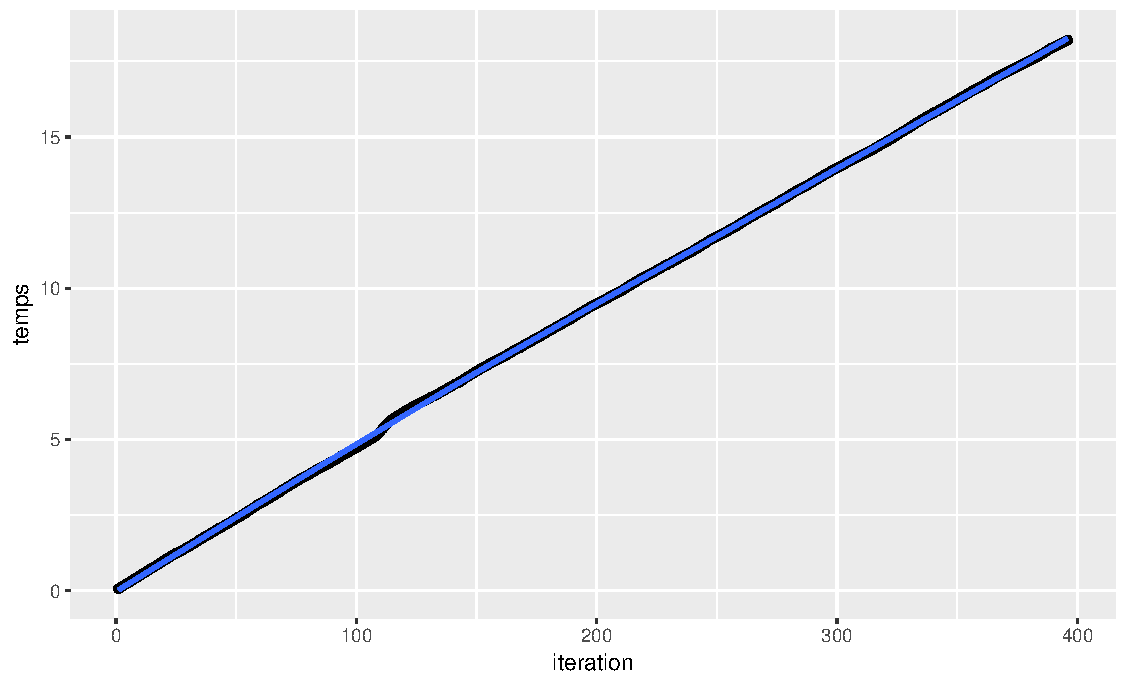
\includegraphics[width = 0.7\linewidth]{plots/tvsiter.pdf}
			\caption{Evolution du temps de calcul en fonction du nombre d'itérations. \label{fig:tvsiter}}
		\end{figure}

		De même, on peut observer sur la figure \ref{fig:tvsm} que la complexité est bien linéaire en fonction de la taille du sous-espace de Krylov comme prédit par la théorie.
		\begin{figure}
			\centering
			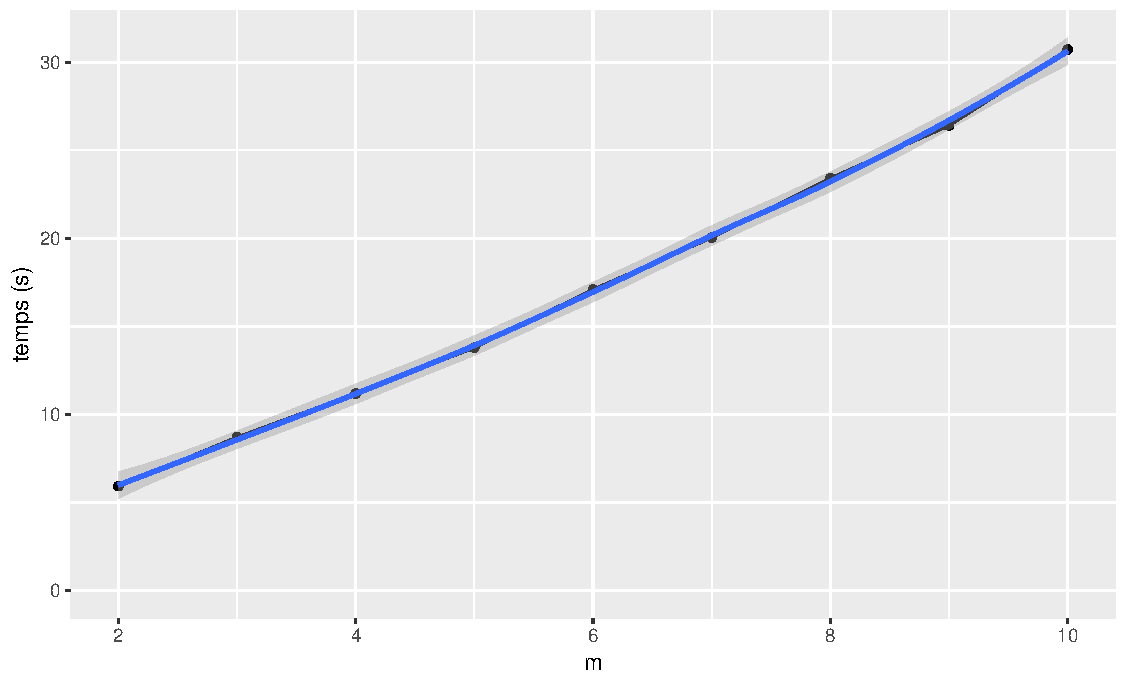
\includegraphics[width = 0.7\linewidth]{plots/tvsm.pdf}
			\caption{Evolution du temps de calcul en fonction de la taille du sous-espace de Krylov $m$. \label{fig:tvsm}}
		\end{figure}

		Finalement, on peut observer sur la figure \ref{fig:tvsM}, qui est en échelle logarithmique, que la complexité suit bien une loi de puissance d'ordre environ 2 en fonction de la taille de la matrice comme prédit par la théorie. Pour réaliser cette figure, nous avons utilisé des matrices de tests possédant la même structure et ayant pour seule différence la taille.
		\begin{figure}
			\centering
			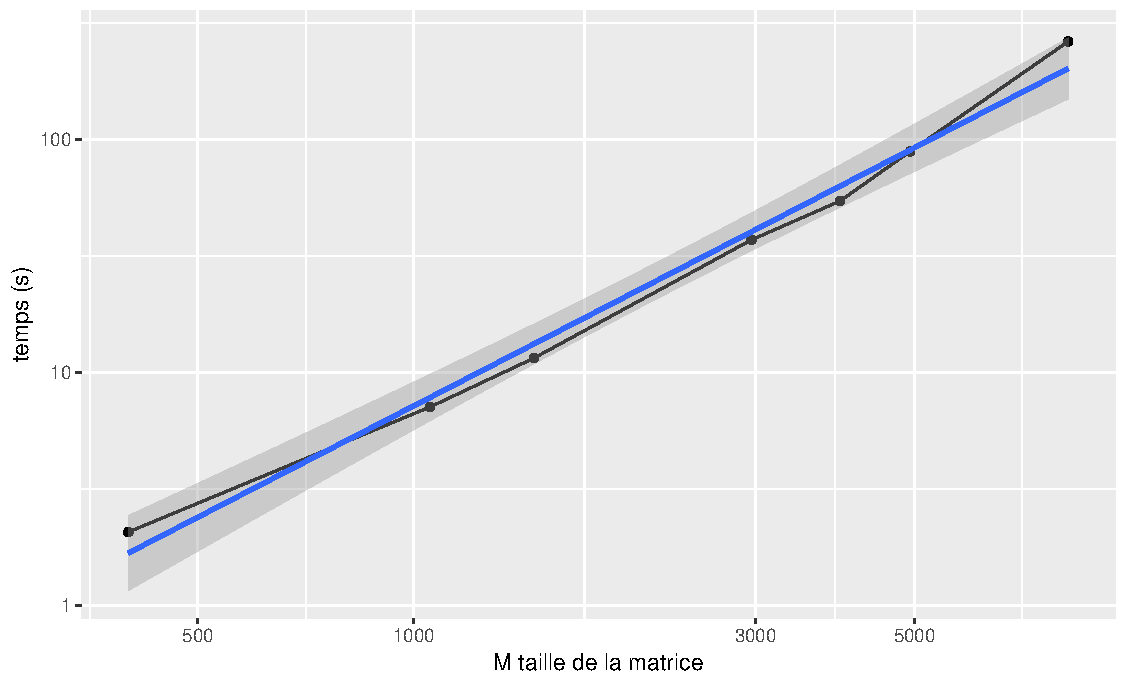
\includegraphics[width = 0.7\linewidth]{plots/tvsM.pdf}
			\caption{Evolution du temps de calcul en fonction de la taille de la matrice $M$. \label{fig:tvsM}}
		\end{figure}


	\subsection{\'Etude de convergence}
		Après avoir étudié les performances de notre implémentation, nous nous intéressons désormais à l'étude de la précision. Pour ce faire, nous étudions notamment la vitesse de convergence de l'algorithme en fonction des différents paaramètres utilisés.

		On peut tout d'abord observer sur les figures \ref{fig:Nvse-m_p6}, \ref{fig:Nvse-m_p8} et \ref{fig:Nvse-m_p10} l'impact du choix de la taille du sous espace de Krylov. Nous nous sommes limités à 10000 itérations, une telle valeur signifie donc une non convergence sur les graphiques. On constate que, de manière générale, une taille de sous-espace de Krylov $m$ plus grande permet une meilleure convergence générale d'un plus grand nombre de vecteurs propres. On peut voir sur la figure \ref{fig:Nvse-m_p10} que seule une taille $m \geq 8$ permet de faire converger 4 vecteurs propres avec une précision $p=\SI{e-10}{}$, pour les valeurs inférieures de $m$ moins de vecteurs propres convergent. On peut néanmoins remarquer sur la figure \ref{fig:Nvse-m_p8} qu'un $m$ inférieur peut permettre une convergence plus rapide. Cela nous montre bien qu'il y a un compromis à trouver pour la valeur de $m$ qui doit être assez grande pour permettre à assez de vecteurs propres de converger mais pas trop grande au risque de perdre en vitesse de convergence dans certains cas.

		\begin{figure}
			\centering
			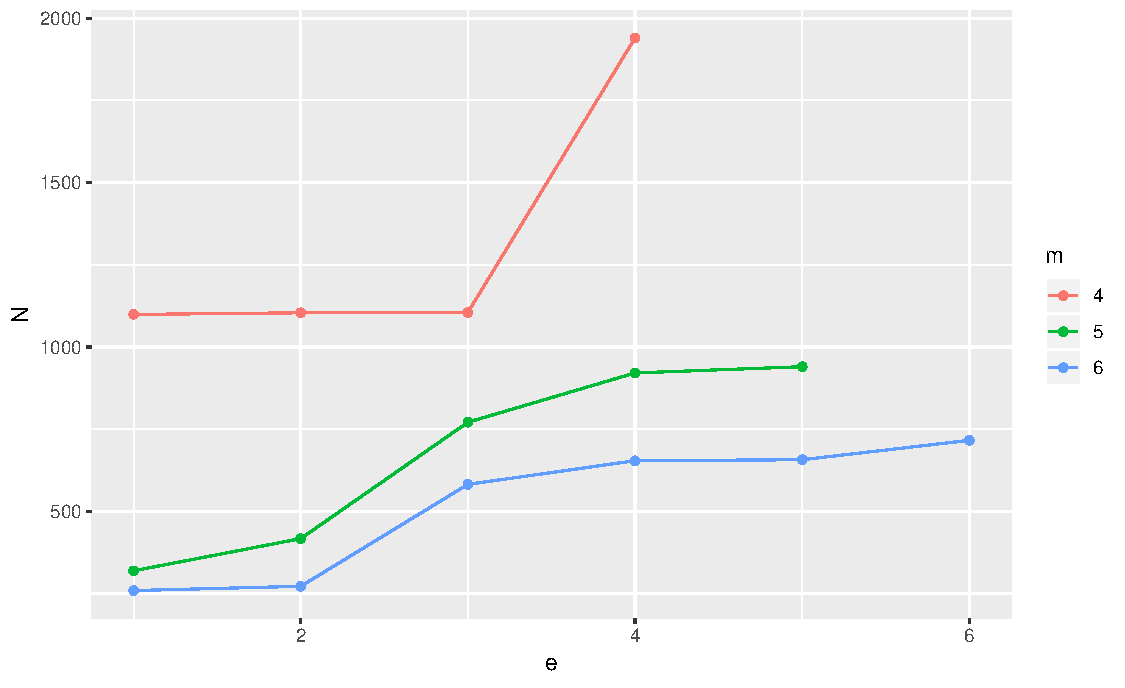
\includegraphics[width=0.8\linewidth, keepaspectratio]{plots/Nvse-m_p6.pdf}
			\caption{Nombre d'itérations $N$ nécessaires pour faire converger $e$ valeurs propres pour différentes tailles de sous-espace de Krylov $m$ et une précision $p=\SI{e-6}{}$ \label{fig:Nvse-m_p6}}
		\end{figure}

		\begin{figure}
			\centering
			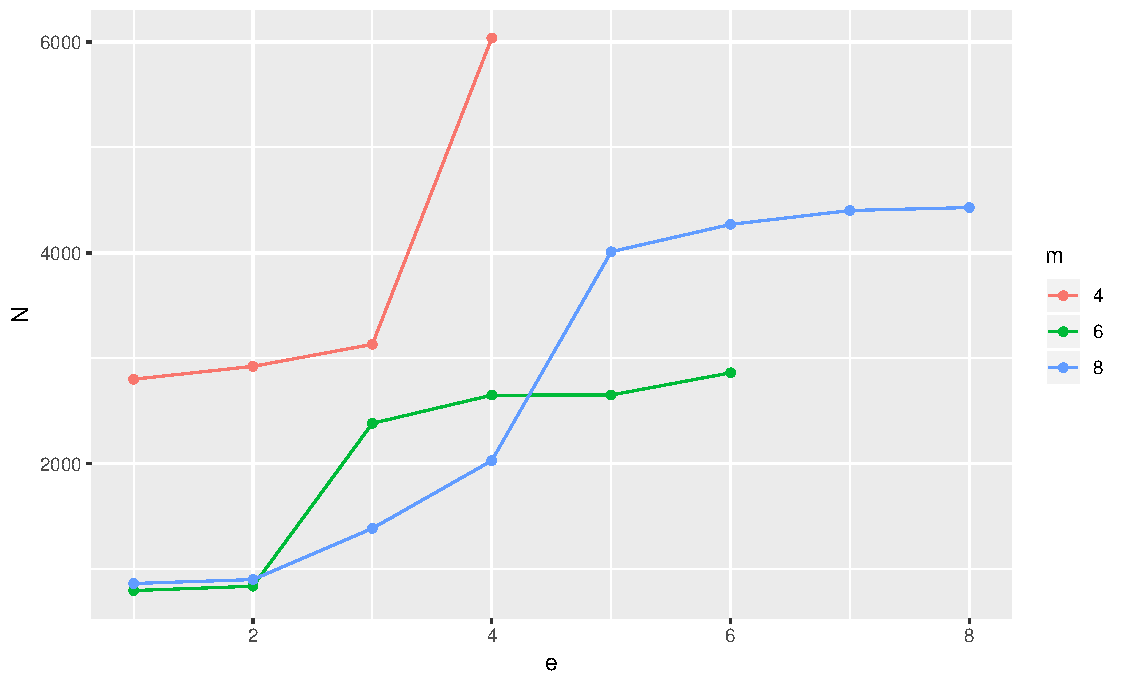
\includegraphics[width=0.8\linewidth, keepaspectratio]{plots/Nvse-m_p8.pdf}
			\caption{Nombre d'itérations $N$ nécessaires pour faire converger $e$ valeurs propres pour différentes tailles de sous-espace de Krylov $m$ et une précision $p=\SI{e-8}{}$ \label{fig:Nvse-m_p8}}
		\end{figure}

		\begin{figure}
			\centering
			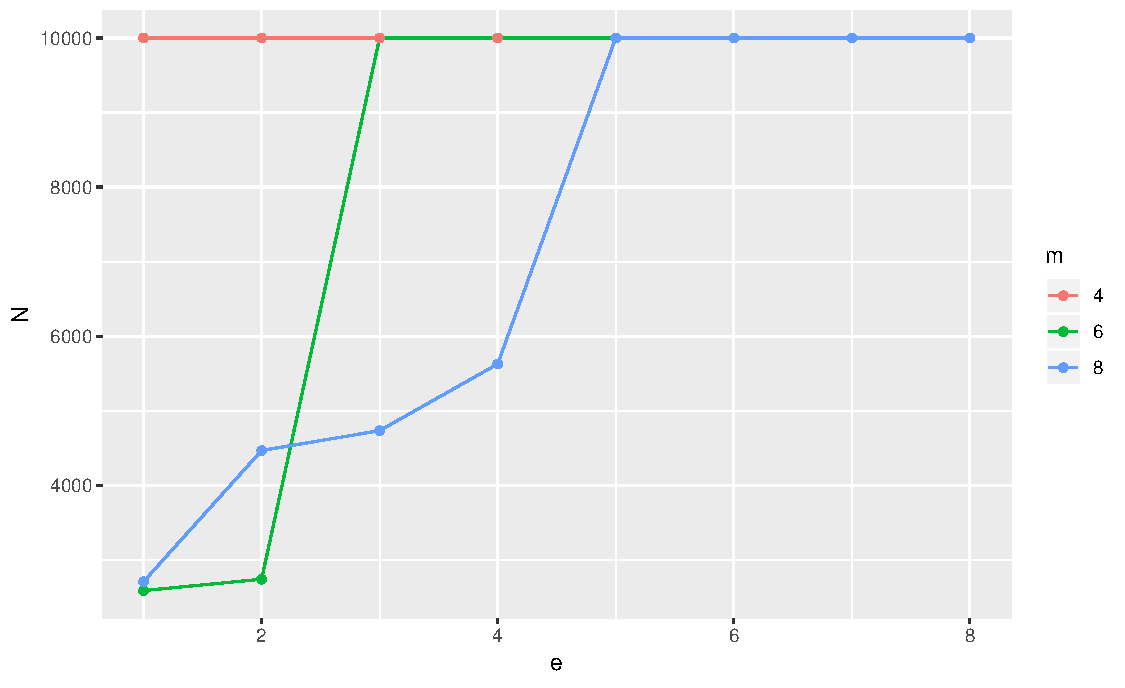
\includegraphics[width=0.8\linewidth, keepaspectratio]{plots/Nvse-m_p10.pdf}
			\caption{Nombre d'itérations $N$ nécessaires pour faire converger $e$ valeurs propres pour différentes tailles de sous-espace de Krylov $m$ et une précision $p=\SI{e-10}{}$ \label{fig:Nvse-m_p10}}
		\end{figure}

		On peut finalement observer sur la figure \ref{fig:Nvsp-m_e4} que le nombre d'itérations nécessaires augmente avec la précision et que la convergence est plus rapide pour une plus grande valeur de $m$. Cela nous montre que la valeur de $m$ à choisir est aussi liée à la précision que l'on désire atteindre.

		\begin{figure}
			\centering
			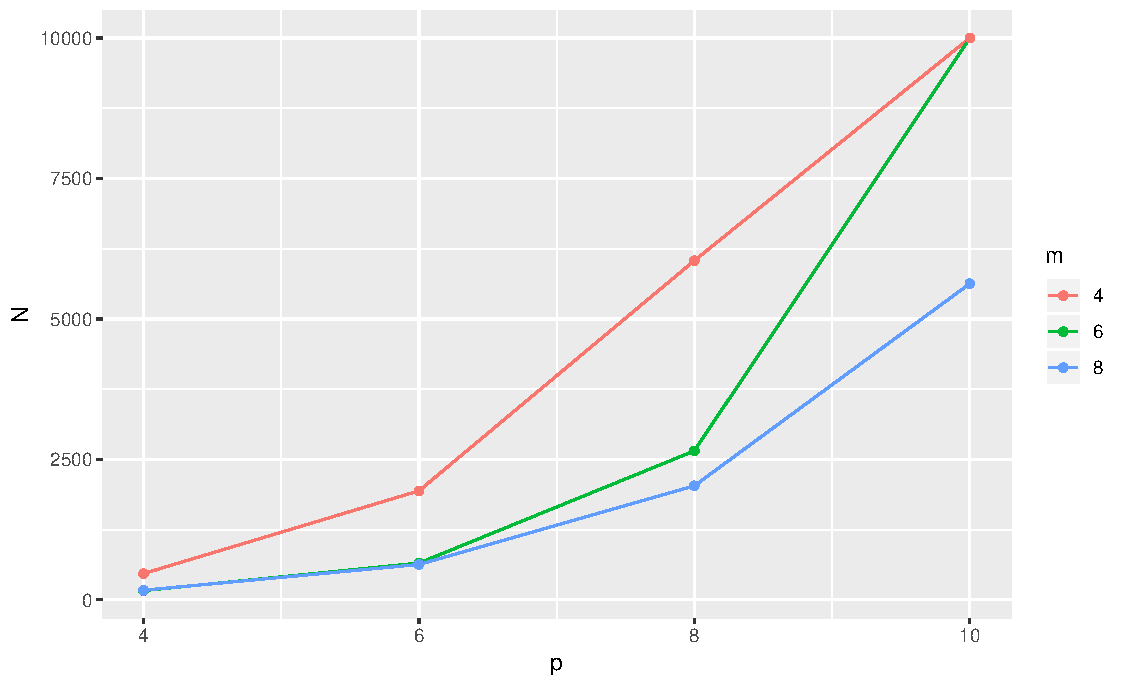
\includegraphics[width=0.8\linewidth, keepaspectratio]{plots/Nvsp-m_e4.pdf}
			\caption{Nombre d'itérations $N$ nécessaires pour faire converger $e = 4$ valeurs propres pour différentes tailles de sous-espace de Krylov $m$ et une précision $p$ \label{fig:Nvsp-m_e4}}
		\end{figure}


	\subsection{Ajout d'une méthode de déflation "Locking"}
		Toutes les valeurs propres de la matrice possèdent une vitesse de convergence différente par la méthode des itérations simultanées. Cela nous amène à affiner et recalculer constamment des vecteurs déjà connus avec la bonne précision ce qui entraine une perte de temps de calcul. De plus, des vecteurs propres qui ont déjà convergés jusqu'à la bonne précision peuvent perdre en précision à cause d'instabilités numériques au fil des calculs : la précision de certains vecteurs propres peut osciller au cours des itérations.

		Afin de résoudre ces deux problèmes nous avons décidé de mettre en place une méthode de déflation appelée "locking". Le principe est simple : lorsqu'un vecteur propre a convergé jusqu'à la précision désirée, on le verrouille de sorte à ne plus le remultiplier par la matrice $A$ et on diminue la taille du sous-espace de Krylov d'une unité. Néanmoins, on utilise toujours ce vecteur pour l'orthonormalisation afin qu'il guide la convergence correcte des vecteurs restants.


		On représente sur la figure \ref{fig:comp_locks} la précision au cours des itérations pour $e$ et $m$ fixés dans le cas de la méthode initiale et de la méthode avec locking. On peut tout d'abord observer que la convergence est bien plus rapide lorsque le locking est utilisé (environ 2000 contre 3800 itérations). On peut en outre constater sur la figure \ref{wlock_e4_p8_m8} que la convergence avec locking semble moins instable.

		\begin{figure}
			\centering
			\begin{subfigure}{0.49\linewidth}
				\centering
				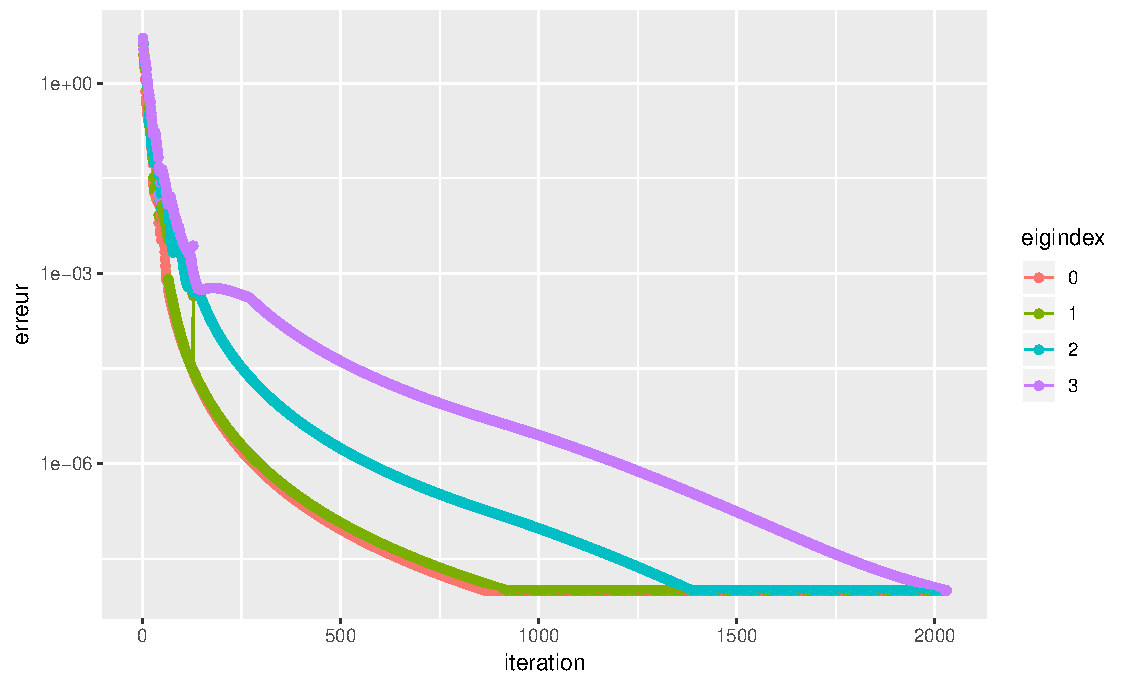
\includegraphics[width=\linewidth, keepaspectratio]{plots/wlock_e4_p8_m8.pdf}
				\caption{Avec locking\label{wlock_e4_p8_m8}}
			\end{subfigure}
			\begin{subfigure}{0.49\linewidth}
				\centering
				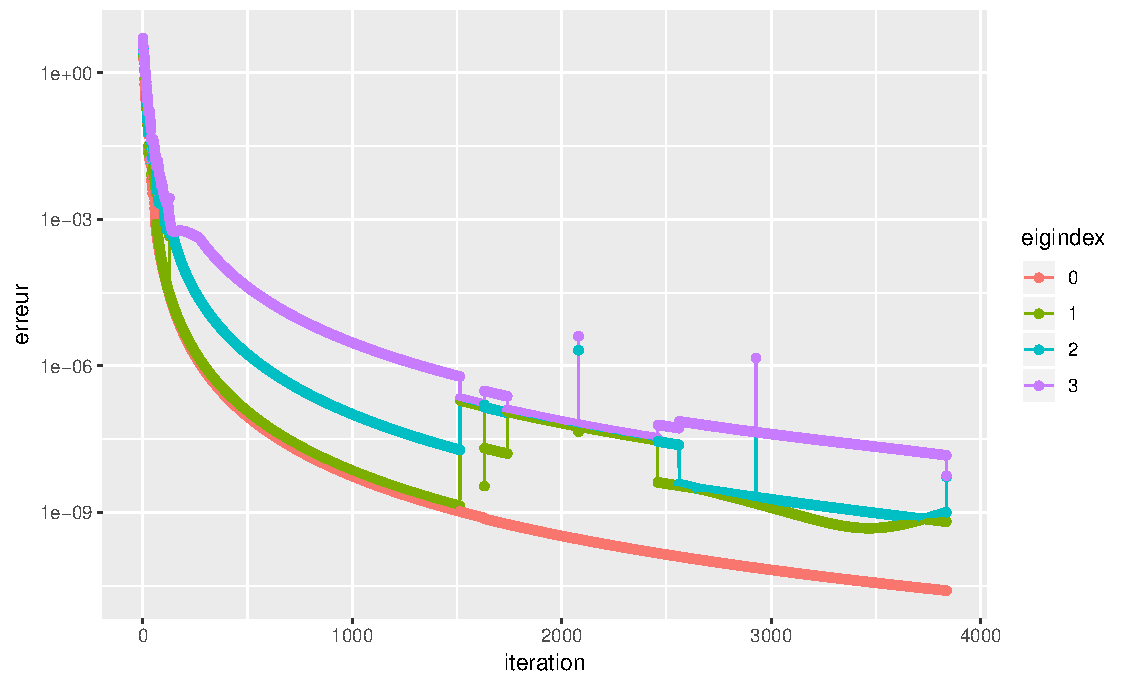
\includegraphics[width=\linewidth, keepaspectratio]{plots/wolock_e4_p8_m8.pdf}
				\caption{Sans locking\label{wolock_e4_p8_m8}}
			\end{subfigure}
			\caption{Précision au cours des itérations $N$ pour $e = 4$ valeurs propres pour une taille de sous-espace de Krylov $m=8$\label{fig:comp_locks}}
		\end{figure}

		De même, on peut voir sur la figure \ref{fig:Nvsp_complock} que l'ajout du locking permet de gagner en rapidité notamment lorsque la précision et la taille du sous-espace de Krylov sont élevés.

		\begin{figure}
			\centering
			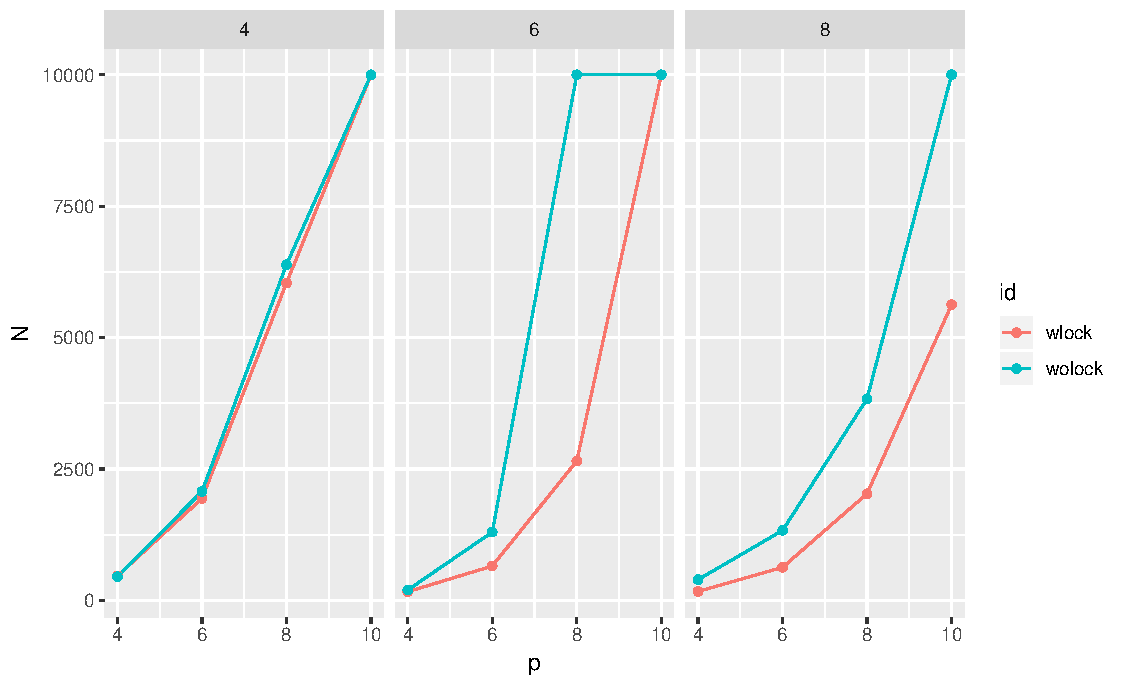
\includegraphics[width=0.8\linewidth, keepaspectratio]{plots/Nvsp_complock.pdf}
			\caption{Nombre d'itérations $N$ nécessaires pour faire converger $e = 4$ valeurs propres pour différentes tailles de sous-espace de Krylov $m$ et une précision $p$ avec et sans utilisation du locking \label{fig:Nvsp_complock}}
		\end{figure}

		En outre, en plus de diminuer le nombre d'itérations, la méthode de locking permet de diminuer la complexité à chaque fois qu'un vecteur est verouillé car on diminue alors la taille du sous-espace de Krylov et ainsi la complexité qui dépend linéairement de $m$.

	\subsection{Conclusions}
		Nous avons pu correctement implémenter l'algorithme des itérations simultanées en séquentiel et retrouver, grâce à nos mesures, la omplexité théorique prédite. Nous avons pu mesurer l'impact des différents paramètres sur la vitesse de convergence de l'algorihme et notamment celle de la taille du sous-espace de Krylov $m$ qui doit être choisi soigneusement. Nous aons par la suite amélioré notre premier algorithme en implémentant le locking ce qui permet d'obtenir une convergence plus rapide et avec une complexité moindre.

\section{Cas parallèle}
	\subsection{Approches utilisées}

	\subsubsection{Approche multic\oe{}urs}

		Maintenant que nous avons correctement pu tester notre code séquentiel et valider les résultats obtenus, nous nous attachons à paralléliser notre implémentation. Tout d'abord, il faut remarquer que nous effectuons des calculs dans deux espaces vectoriels différents : dans l'espace d'origine $\mathbb{R}^{N\times N}$ et dans le sous-espace de Krylov $\mathbb{R}^{m\times m}$. Les calculs les plus couteux sont donc bien évidemment ceux effectués dans l'espace d'origine qui est une dimension largement supérieure à celle du sous-espace de Krylov. Les calculs qu'il est donc nécessaire de paralléliser sont ceux effectués dans l'espace d'origine ainsi que les changements de base pour passer de l'espace d'origine au sous-espace de Krylov. Les calculs à paralléliser sont donc les produits matriciels dans l'espace d'origine.

		Afin de paralléliser les produits matriciels, on commence par l'implémentation la plus simple et la plus efficace qui consiste à effectuer une parallélisation en mémoire partagée grâce à \textbf{OpenMP}. En effet, la plupart des calculs sont indépendants lors du produit matriciel et l'on peut gérer efficacement les réductions. De plus, puisque la mémoire est partagée, il n'y a pas de pénalités de communication. On réalise cet ajout d'OpenMP à l'aide d'instructions pragmas devant les boucles qui peuvent être parallélisées.
		
		\subsubsection{Approche multi-n\oe{}uds}

		Une fois que nous avons pu exploiter les différents c\oe{}urs d'un n\oe{}ud, il est nécessaire pour augmenter encore les performances d'utiliser les différents n\oe{}uds du cluster. Pour cela on utilise \textbf{MPI}. Les produits matriciels représentant de loin la part dominante du temps de calcul, nous avons décider de distribuer ces opérations.

		Nous avons pour cela implémenté un algorithme basique pour $n$ nœuds comprenant un n\oe{}ud principal et $n-1$ esclaves :

		\begin{itemize}
			\item Hors produit matriciel : le n\oe{}ud principal s'occupe de l'intégralité des opérations.
			\item Lors d'un produit matriciel $C = AB$, le n\oe{}ud principal communique les matrices $A$ et $B$ au autres n\oe{}uds. Chaque n\oe{}ud, y compris le n\oe{}ud principal effectue le calcul d'une sous-matrice de $C$ et communique cette matrice au processus principal qui reconstruit $C$.
		\end{itemize}

		\paragraph{Remarques :}
		\begin{itemize}
			\item On utilise la fonction \texttt{MPI\_BROADCAST} qui permet d'envoyer les matrices $A$ et $B$ lors d'une unique communication à tous les n\oe{}uds esclaves.
			\item On peut réduire l'envoi de la matrice $A$ au lignes qui sont utilisées par le n\oe{}ud esclave.
		\end{itemize}

	\subsection{Étude de performances théorique}

		\subsubsection{Approche multic\oe{}urs}

		En utilisant OpenMP en mémoire partagée pour un n\oe{}ud de $N$ c\oe{}urs, on atteint théoriquement un accélération égale à $N$. On suppose en effet que l'on peut négliger les effets d'overhead introduits par OpenMP car les boucles parallélisées sont très longues.

		On a donc un temps d'exécution divisé par le nombre de c\oe{}urs.

		\subsubsection{Approche multi-n\oe{}uds}

			Considérons le produit matriciel $C = AB$ avec des matrice carrées de taille $n$. Cela est généralisable à des matrices rectangulaires.

			On étudie l'accélération théorique en passant de l'utilisation d'une unique n\oe{}ud à l'utilisation de $N$ n\oe{}ud grâce à MPI.
			\paragraph{Conséquence sur le temps de calcul des produits matriciels :}
				Chaque c\oe{}ur calcule $\frac{1}{N}$ de la matrice C, on divise donc par $N$ le temps de calcul d'un produit matriciel.

			\paragraph{Impact du temps de communications}
				Les n\oe{}uds MPI doivent avant et après chaque produit matriciel échanger les matrices concernées avec le n\oe{}ud principal. On a les échanges suivant avec le n\oe{}ud principal :
				\begin{itemize}
					\item \textbf{Avant} : Toute la matrice B en broadcast
					\item \textbf{Avant} : $\frac{1}{\sqrt{N}}$ de la matrice A pour chaque processus
					\item \textbf{Après} : $\frac{1}{N}$ de la matrice C pour chaque processus
				\end{itemize}

				On communique uniquement $\frac{1}{\sqrt{N}}$ de la matrice A pour chaque processus car le calcul de la sous-matrice $C_{i..k,j..l}$ nécessite les sous-matrices $A_{i..k,0..n}$ et $B_{0..n,j..l}$. Comme les matrice sont stockées par ligne dans notre programme nous n'avons pu faire cette optimisation que pour la matrice A, la matrice B étant donc envoyée en broadcast.

			On a un temps d'exécution théorique qui est le temps de calcul divisé par $N$ additionné au temps de communication.

			$$
			\fbox{$t^{par} = \frac{t^{seq}}{N} + t^{com}$}
			$$

			Avec
			\begin{itemize}
				\item $t^{par}$ temps d'exécution du produit matriciel avec MPI
				\item $t^{seq}$ temps d'exécution du produit matriciel sans MPI
				\item $t^{com}$ temps de communication lors du calcul matriciel

			\end{itemize}
			

	\subsection{Étude de performances pratique}

		\subsubsection{Approche multic\oe{}urs}
		
			Les gains en performance apportés par OpenMP sont représentés sur la figure \ref{fig:omp_perf}. On peut observer que l'on gagne un facteur 7 d'accélération en utilisant 8 cœurs physiques ce qui est très important. Cela montre que notre code est fortement parallélisable, c'est à dire que les parties séquentielles ne représente qu'une petite proportion du temps de calcul. On peut ensuite observer sur la figure que lorsque l'on utilise des cœurs logiques hyperthreadés supplémentaires les performances sont dégradées avant de s'améliorer lorsque leur nombre augmente. Ceci est logique car les cœurs hyperthreadés ne possèdent pas leurs propres modules pour effectuer les opérations et ne proposent donc pas une bonne accélération lorsque le code est fortement parallélisable.

			\begin{figure}
				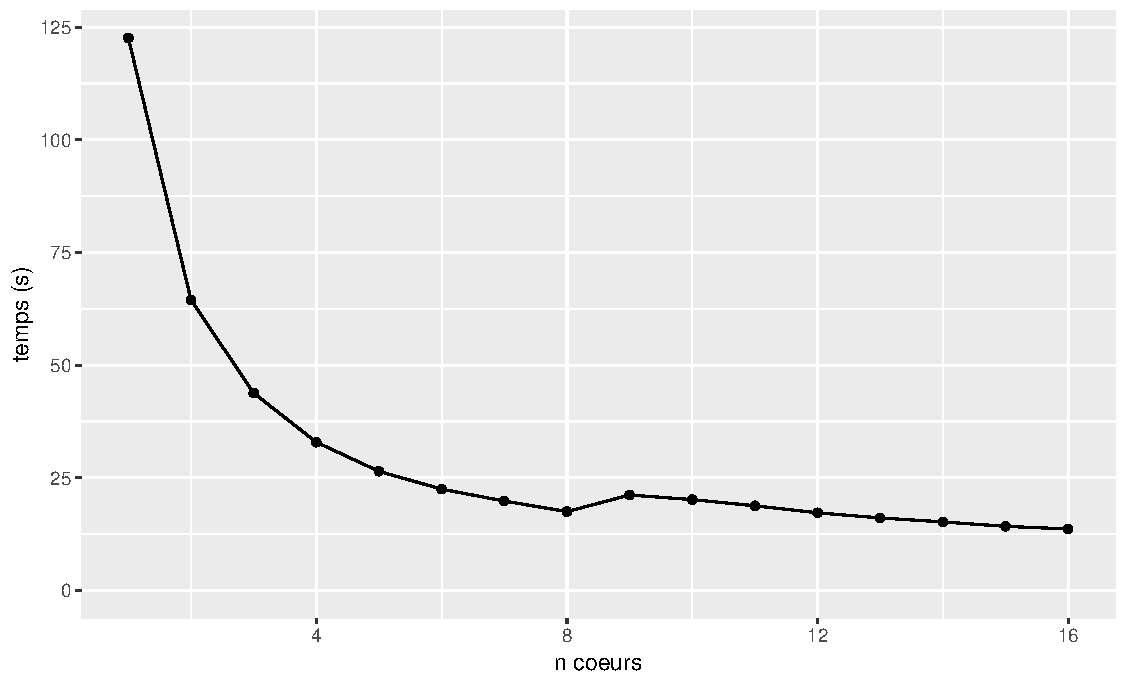
\includegraphics[width=\linewidth]{plots/omp_perf.pdf}
				\caption{Évolution de l'efficacité de l'implémentation en fonction du nombre de threads OpenMP utilisés sur un nœud avec 8 cœurs hyperthreadés pour un calcul de 4 valeurs propres avec $m = 8$ à $p=\SI{e-8}{}$ \label{fig:omp_perf}}
			\end{figure}

		\subsubsection{Approche multi-n\oe{}uds}

			Le tableau de la figure \ref{res-mpi} donne les résultats de l'exécution de programme avec l'utilisation de plusieurs n\oe{}uds. Deux matrices carrées différentes ont été utilisée : la première de taille 1473 et la deuxième de taille 4929. Toutes deux proviennent de la base Matrice Market.

			\medskip
		
			Les grandeurs renseignées sont les suivantes :
			\begin{itemize}
				\item taches : Nombre de processus MPI lancés.
				\item n\oe{}uds : Nombre de n\oe{}uds du cluster réservés.
				\item N : Taille de la matrice.
				\item threads : Nombre de threads OpenMP configurés.
				\item M : Taille du sous-espace de Krylov.
				\item temps : Temps d'exécution total du programme en secondes.
			\end{itemize}

			\begin{figure}
				\begin{center}
					\begin{tabular}{l l l l l l}
						taches	& noeuds & N & threads & M & temps (s)\\ \hline
						1 		& 1 & 1473 & 16 & 10 & 4.899005\\
						4 		& 4 & 1473 & 16 & 10 & 9.844218\\
						6 		& 1 & 1473 & 16 & 10 & 66.033455\\ \hline
						1 & 1 & 4929 & 16 & 10 & 29.481719\\
						4 & 4 & 4929 & 16 & 10 & 82.517647\\
					\end{tabular}
				\end{center}
				\caption{Résultats de l'exécution de la version MPI du programme sur le cluster Poincaré}
				\label{res-mpi}
			\end{figure}

			\bigskip

			On observe que lorsqu'on utilise plusieurs n\oe{}uds le temps d'exécution augmente de manière importante. On peut penser qu'une telle baisse de performances en multi-n\oe{}uds provient de l'ajout de communications pour l'échange des matrices. Un piste pour rendre cette algorithme MPI réellement efficace serait d'optimiser les échanges de matrices.

	\subsection{Conclusions}

	La parallélisation via OpenMP donne de très bons résultats sans avoir à modifier le code. Cela vient notamment de la présence d'une mémoire partagée. Néanmoins les n\oe{}uds de cluster on un nombre de c\oe{}urs physiquement limité, ce qui conduit à implémenter des solutions MPI pour augmenter encore les performances.

	A l'inverse la parallélisation MPI demande des modifications structurelles du code et ne donne pas de résultats immédiats notamment à cause du grand surcoût des communications de grandes matrices.

\section{Conclusion générale}

	Nous avons pu implémenter la méthode des itérations simultanées afin de calculer les valeurs et vecteurs propres d'une grande matrice creuse. Nous avons ensuite tenté d'améliorer l'algorithme initialement proposé en introduisant le "locking" permettant de modifier les paramètres de redémarrage afin de gagner à la fois en temps de calcul et en stabilité numérique de la convergence. Nous avons pu constater que l'ajout du locking a effectivement permis d'augmenter l'efficacité et la précision de notre implémentation. Nous avons aussi implémenté un conditionnement simpliste des matrices en entrée afin de résoudre certains problèmes de stabilité numérique dans le cas de matrices mal conditionnées en entrée.

	Nous nous sommes ensuite proposés de paralléliser notre programme à l'aide de deux outils : OpenMP et MPI. Nous avons tout d'abord effectué la parallélisation des boucles avec OpenMP puis nous avons implémenté les produits de matrices couteux en MPI. Nous avons pu tester notre code parallèle sur le cluster poincare à la maison de la simulation. Les résultats furent assez décevants car notre parallélisation MPI a augmenté les temps de calcul à cause des coups trop élevés des transferts de données. Nous en concluons que la parallélisation efficace de ce type d'algorithme doit plutôt reposer sur l'implémentation de méthodes hybrides.

\end{document}
